In the previous chapters, many different methods that can be used to compute PESs numerically are described and in chapter \ref{ch:proced} the method used within this work is described in more detail.
In this chapter some results are shown and explained.

Since the method developed in this work combines several techniques that have not been used together so far and several conceptual questions need to be clarified before computing actual PESs, is section \ref{ch:BCbench} three boundary conditions are compared in their influence on the wave-function. In section \ref{sec:NumConve} further benchmarking calculations on some numerical parameters are shown.
For simplicity, these calculations were performed using a Lithium atom as test system.

In section \ref{ch:resLI} further results for atomic Lithium are presented, showing several conceptual ... .

%There is a paper\cite{vibPES} with vibronically resolved PES from experiment.\\
%PES of N2 with 'angular resolution' (latter not directly) \cite{PESN2}.
%purine and pyrimidine: comparison to Green's function methods via the \cite{PottsHolland}-paper.
%For AlO$^-$ there is a paper with 2 spectra with one and two transitions each, having vibrational
%structure\cite{AlO}.
%Atomic Systems have some experimental data as well: For Xe and Kr the spectra at photon energies of 150$\,$eV are shown in reference \cite{KrXe}.
%A combined theoretical and experimental study on CH$_2$F$_2$ is in ref. \cite{ch2f2}. Here, theory is quite bad and experiment is also angular resolved, thus may be interesting.

\section{Comparison of Boundary Conditions}
\label{ch:BCbench}
In section \ref{ch:BC} many boundary conditions were introduced briefly which give rise to diverse properties for the solution which are studied in various works for several systems \cite{babuska}.
Since in general the design of proper boundaries is sufisticated, no comprehensive investigation on this is given.
Instead, a few results obtained with Dirichlet boundaries, CAPs and infinite elements are compared and some main characteristics should be found.

\subsection{Dirichlet Boundary Conditions}
Study the behaviour of solutions with box-size.\\
Mainly look at DOS and spherical partial waves.

\subsection{Complex Absorbing Potential}
Study the behaviour for different distances and strengthes for two box-sizes (smallest reasonable, larger one?)

\subsection{Infinite Elements}
Several questions and conceptual problems have been posed in the previous chapters which require some investigation to get an understanding of the properties of the numerical setup described so far.
Among these questions is the formulation of infinite elements, discussed in section \ref{ch:InfEl} of which the most important ones are studied in section \ref{ch:bmFormul}.

Another important question concerns the scheme to be used for the setup of the mesh: In section \ref{sec:grid} the properties of obtained FEFs depending on the grid-parameters are studied.

%\subsubsection{Formulation of Infinite Elements}
\subsubsection{Comparison of Formulations}
\label{ch:bmFormul}
While the unconjugated Burnett-formulation was not very successfull, the conjugated formulations of Burnett and Astley-Leis both have interesting features to use for quantum mechanical problems.
Since the conjugated Burnett elements lead to infinitely large matrix elements, here the Astley-Leis elements (\ref{eq:ALelem}) are compared with the symmetrised form (\ref{eq:ALsymm}) using different powers $p$.
Moreover, to study the influence of the damping function in the Astley-Leis formulation (\ref{eq:ALelem}) in more detail, also a test function space similar to eq. (\ref{eq:ALelem}) but using the squared damping function $D(r)^2$ instead of $D(r)$.

The 50 real solutions whose energy is closest to the target value of $15.44\,$eV ($0.5675\,E_h$) obtained with the original Astley-Leis formulations with the damping function taken to the powers $p=1,2$ as well as the symmetrised formulation (\ref{eq:ALsymm}) suggested in this thesis with powers $p<0.5$ are shown in Figure \ref{fig:IFEMform_spect}.
For the unsymmetric formulations only the real part is shown which is assigned to the physical energy of the respective state.
\begin{wrapfigure}{r}{0.65\textwidth}
\includegraphics[width=0.65\textwidth]{Figures/IFem_form_spectra}
\caption{The first 50 eigenvalues obtained with the original Astley-Leis formulation (imaginary part not shown) and with the symmetrised form (\ref{eq:ALsymm}).}
\label{fig:IFEMform_spect}
\end{wrapfigure}
The results shown in Figure \ref{fig:IFEMform_spect} show clearly that the obtained density of states decreases with the power $p$ and converges for $p\approx \frac 18$ for the given parameters (the radial mapping scheme (\ref{eq:tm_map}) is used with $N=25$, $l=0.5$, $p=2.5$ and $r_\text{max}=7\,$bohr.).

The dependence of the obtained spectrum of the Hamiltoninan on the power of the damping function shows that, at least for FEFs, the asymtotic behaviour is crucial for the properties of thp wave function. 
Moreover, even for small powers $p\approx 10^{-4}$, no numerical instabilities are observable so that there is some freedom in this parameter and it does not need to be optimised for different systems individually.
The observations made on the convergence-properties using the spectrum in Figure \ref{fig:IFEMform_spect} are supported by the projections of the solutions on spherical waves of which some are shown in Figure \ref{fig:IFEMform_project}.
\begin{figure}
\includegraphics[width=\textwidth]{Figures/Ifem_forms}
\caption{Decomposition of the first 30 solutions into spherical waves with anular momenta up to $l=7$.
Left: Astley-Leis-formulation ($p=1$), middle: symmetrised form ($p=0.5$) right: symmetrised form ($p=10^{-4}$).}
\label{fig:IFEMform_project}
\end{figure}

As shown in the Figure \ref{fig:IFEMform_project}, the nature of the states obtained is in all cases strongly mixed in the quantum number $l$ with significant contributions even for $l>7$.
However, the relative contributions of the angular momenta critically depends on the power $p$, making a reasonable choise of this parameter important.

\subsubsection{Radial Order}
The order of radial polynomial: Show graph similar to \ref{fig:IFEMform_spect} for this to see convergence.
\textcolor{red}{Show 1-D and 2D cuts through solutions as function of $p$!  (What kind of box?)}

\subsubsection{Order of Integration}
unstable with respect to purely numerical parameters which should converge fast.

\subsubsection{Conclusion on Boundary Conditions}
\begin{itemize}
  \item Dirichlet BC: very slowly converging with box-size, radial function very poorly estimated for small boxes.
       But good convergence properties, eigenstates of angular momentum.
  \item CAP: algorithmic scheme to find single best energy, but not straight-forward to find some clear scheme if many solutions (have) to be taket into account.
  \item infinite elements: from theory point best conditions but show chaotic behaviour due to almost-degeneracy in analytical subspace No algorithmic procedure known to finde best parameters.
\end{itemize}
Results in the non-intuitive conclusion that less accuracy leads to better results.

%\subsection{Hamiltonian dependence on wave vector}
%Due to the inifinite elements, the Hamiltonian depends on the target momentum $k$ as can be seen in eq. (\ref{eq:SymmKinE}) and (\ref{eq:InFEMmatrix}).
%The nature of this dependence of especial interest since it is a special characteristic of this formulation and another numerical parameter influencing the solutions.
%\begin{wrapfigure}{r}{0.5\textwidth}
%\includegraphics[width=0.5\textwidth]{Figures/E_k_benchmark}
%\caption{Energies of the solutions obtained for target energies varying in the $\mu\,E_h$-range.}
%\label{fig:E_k_bm}
%\end{wrapfigure}
%The obtained energies of the solutions vary strongly when changing the target momentum $k$ as the Figure \ref{fig:E_k_bm} illustrates.
%In the figure, the target energy is varied between $0.566451\,$a. u. and $0.066551\,$a. u. and lead to strongly changing eigenenergies.
%This strong dependence on $k$ is also observed when projecting the obtained FEFs onto spherical waves (\ref{eq:spherWave}) which is not shown here.

\subsection{Mesh-Construction and Quality}
\label{sec:NumConve}
In section \ref{sec:grid} several parameters for the setup of the grid were discussed whose numerical properties are te compared and evaluated in this section.
Here, three different schemes for distritributing the concentric spheres are presented for the Lithium atom, each with a maximum radius $r_\text{max}=7\,$bohr and $N=20$ spheres.
In the scheme denoted in Table \ref{tab:RadScheme} and Figure \ref{fig:SchemHist} (left) as ``const'', the spheres are placed according to eq. (\ref{eq:tm_map}) with $N_i=74$ points on each sphere.
The scheme denoted as tm also uses eq. (\ref{eq:tm_map}) for the size of respective spheres but adapts the number of points per sphere according to (\ref{eq:tm_num}).
The last scheme tested here uses the radial mapping suggested by Son and Chu \cite{Son_Chu0} (\ref{eq:son_map}) and the number of points per sphere (\ref{eq:son_num}).
The parameters for the radial mapping are chosen as $l=1.8$ and $p=2.6$ and for the distribution of points on the spheres the Lebedev-scheme \cite{lebedev} is used, respectively.
\begin{table}
\begin{tabular}{|c|c|c|c|}
\hline
scheme & runtime [s] & DOS$^{a)}$ [$(m E_h)^{-1}$] & number of nodes\\
\hline
const   &  438   &    7    &   3255 \\
tm      &  825   &    13   &   5132 \\
son     &  891   &    4    &   6368 \\
\hline
\end{tabular}
\caption{The runtime, density of states and number of nodes used for the different radial mapping schemes that are described in the text.\\
$^{a)}$: density of states, averaged over 23 states}
\label{tab:RadScheme}
\end{table}
Some characteristic properties of the respective results are shown in Table \ref{tab:RadScheme}.
The runtime given in this table is only a rough estimation but seem to scale directly proportional to the number of nodes.
Seemingly the radial mapping scheme (\ref{eq:tm_map}) in combination with the angular density (\ref{eq:tm_num}) seems to be advantageous compared to the others even though it should be noted that this may be different for other parameters and that the density of states in these calculations is not uniform so that an average over more or fewer states can influence the results qualitatively.
However, the results may be very sensitive with respect to the change of parameters such as box-size and the parameter $l$, respectively.
Moreover, during the creation of tetrahedra from the given point-sets a quality-check is done by the respective library \cite{tetgen} which adds or removes points to ensure well-shaped tetrahedra which may, however, alter the distributions considerably.
These corrections of the point-set may be also responsible for the very similar distribution of the properties of the different tetrahedra.
In Figure \ref{fig:SchemHist} (left), the distribution of the ratio of the longest edge to the height of the smallest side is shown.
Here no significant differences between the schemes under investigation can be seen.

The angular distribution of points seems to be only of minor importance.
As shown in the Figures \ref{fig:SchemHist} and \ref{appFig:SchemHist} in supplement, the statistics are very similar and also the obtained density of states is very comparable.
However, the angular distribution can play a larger role when considering non-spherical systems.
In this work unless otherwise noted, the Lebedev scheme is used which provided the highest density of states (DOS) in this test.
The impression of very similar properties of the meshes generated by different schemes is also supported by the statistics of further parameters of the tetrahedra, see Figure \ref{appFig:SchemHist}.
\begin{figure}
\includegraphics[width=0.49\textwidth]{Figures/Radi_hist.pdf}
\includegraphics[width=0.49\textwidth]{Figures/Sph_hist.pdf}
\caption{Distribution of aspect ratio (longest edge length divided by the smallest side height).
   Be aware that the ranges of the different bins differ.}
\label{fig:SchemHist}
\end{figure}
Concluding one can say that the procedures studied here yield meshes with similar quality.

\subsection{Numerical Convergence}
In the FEM scheme used to compute the FEF, several parameters governing numerical and physical characteristics are used such as box-size, target energy and subspace used for solving the eigensystem.

The size of the Krylov-subspace does not play a role for the quality of the solution as shown in Figure \ref{fig:E_nev} for the symmetric formulation with a power $p=\frac 12$ of the damping function $D$.
\begin{wrapfigure}{r}{0.5\textwidth}
\includegraphics[width=0.5\textwidth]{Figures/Root_E_nev.pdf}
\caption{The energies of the 20 states that fit the target energy best, depending on the
size of the Krylov-suspace, indicated by the colour.}
\label{fig:E_nev}
\end{wrapfigure}
Such a good behaviour can, however, only be observed for the symmetric case because in case of the non-hermitian formulation the ordering of the eigenvalues can not be done unambiguously.

\subsection{Size of Finite Element Region}
\subsubsection{Radius of the Region}
\label{ch:bmSize}
More important than the subspace used numerically is obviously the size of the sphere used for the FEM description.
\begin{itemize}
   \item `Convergence' speed depends on power of $D$, chose $p= 0.001$ here.
   \item Increasing box-size leads to contributions of larger $l$ 
   \item Non-symmetric formulation leads to stronger mixing of angular momenta
   \item Spectra converged for $p=1/8$, see Figure \ref{fig:powerSpect} in supplement.
\end{itemize}
\begin{figure}
\includegraphics[width=\textwidth]{Figures/RadWave_p0_001.pdf}
\caption{The eigen energies for different box sizes (coloured dots in the upper pannel) where the box size is denoted by the colour in atomic units.
The lower pannel shows the decomposition of the solutions into spherical waves for three box sizes, marked by a star in the color bar respecively.}
\label{fig:RadWaves}
\end{figure}

\subsubsection{Density of Spheres}

\section{atomic Lithium}
\label{ch:resLI}
As the smallest system that has multiple electrons in its anionic state as well, Lithium is a good test object that has theoretical as well as experimental reference data available, \cite{Li-R,Li-R1, LiNaRef1} even though its appearence in a work on `complex molecules' might surprise.
However, its photoelectron spectrum consists, except for a single valence peak, only of the core electron spectrum.
In this region the estimated binding energies are often not that good as those obtained for valence orbitals and, moreover, two out of four main peaks of the spectrum arise due to dipole-transitions in the bound part and thus are not accounted for due to the neglect of the conjugated Dyson orbital in eq. (\ref{eq:fullDO}) \cite{saPonzi}.
%The appearance of $2p$-states are accessed by a dipole-transition in the bound part and can not be described within the theory applied here due to the neglect of the conjugate DO term in equation (\ref{eq:fullDO}) \cite{saPonzi}.
%Experiment from Moore, cited in \cite{LiNaRef1}; original not found.
%Experiment 2 from \cite{LiSonntag}.
%
%\begin{wrapfigure}{l}{0.7\textwidth}
%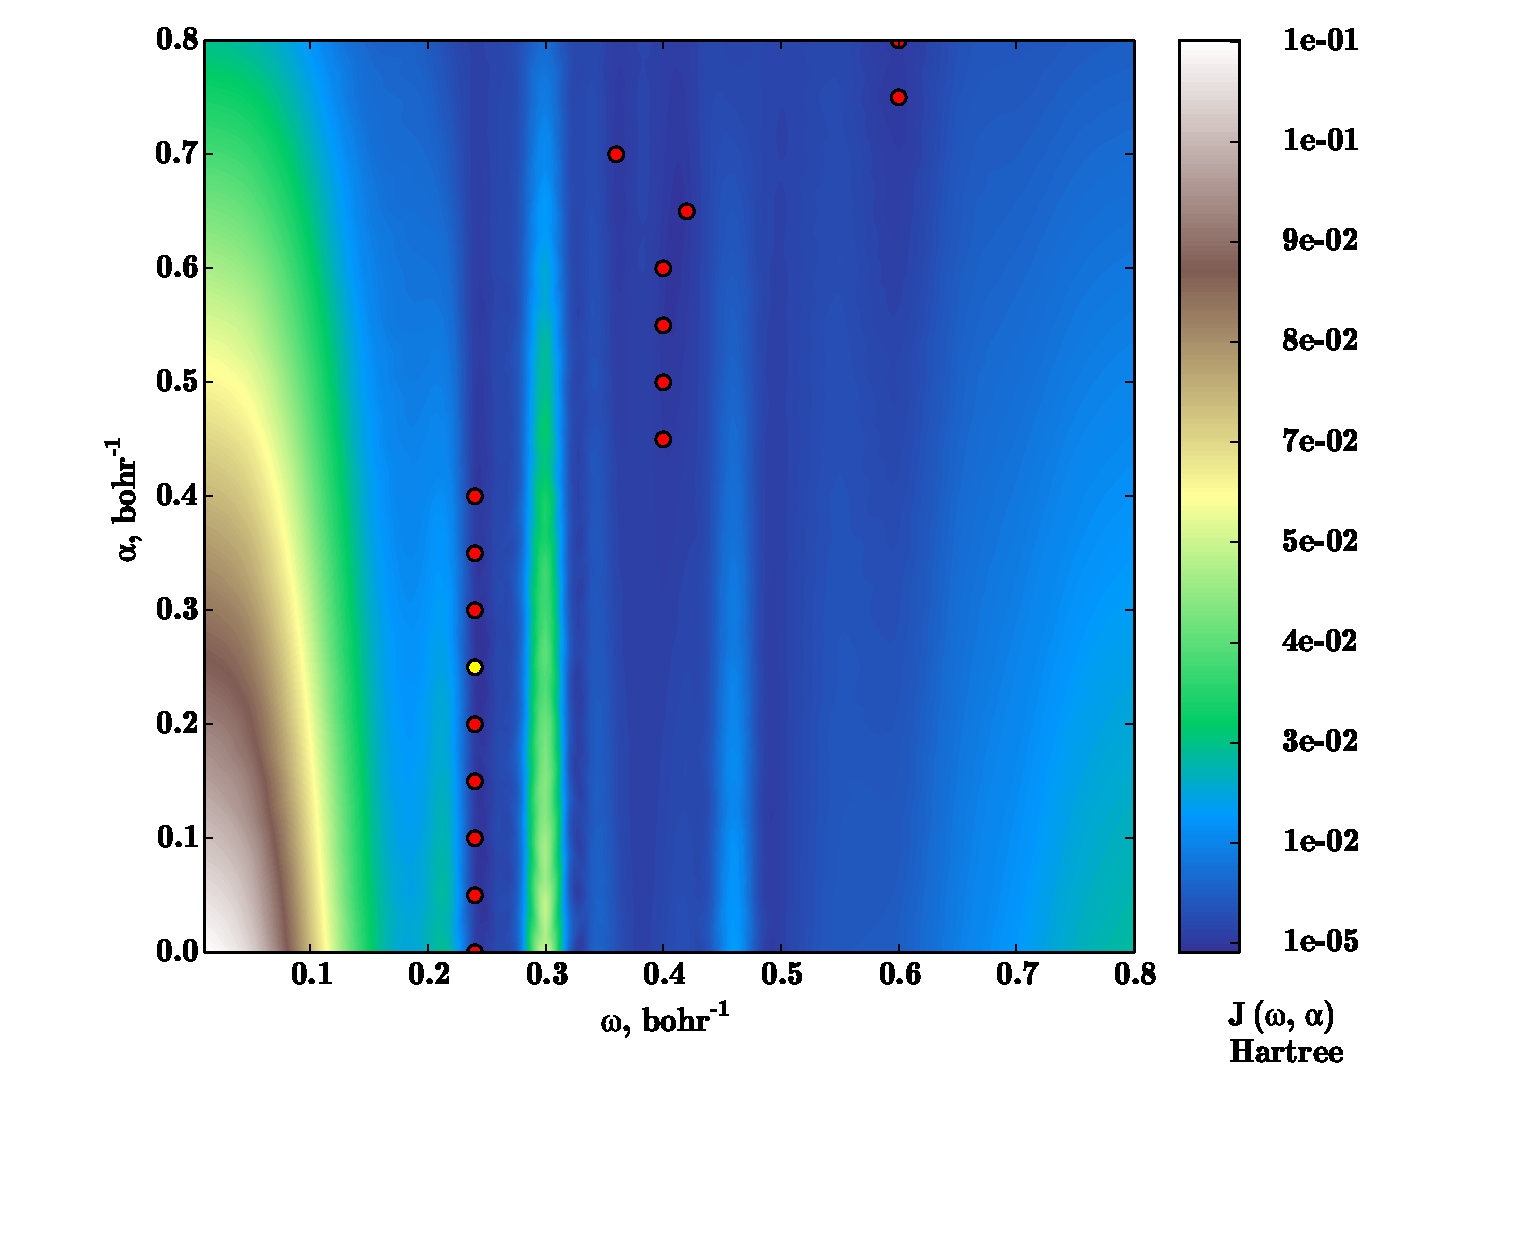
\includegraphics[width=0.69\textwidth]{Figures/Lithium/Lithium_J0_2D_terrain_path_spline_cut}
%\caption{The functional $J(\alpha,\omega)$ described in eqation (\ref{eq:J_ao}) for Lithium}
%\label{fig:Lith-otrsh}
%\end{wrapfigure}

However, the well-separated single valence peak allows a more detailed study of the photon energy dependence of the intensity of a single peak as shown in Figure \ref{fig:Lith-cs} where experimental values are compared with several theoretical models.
\begin{wrapfigure}{l}{0.7\textwidth}
\includegraphics[width=0.69\textwidth]{Figures/Lithium/Li_crossSect}
\caption{Cross section of the Lithium atom as function of the photon energy \cite{LiCS}.}
\label{fig:Lith-cs}
\end{wrapfigure}
Since the protocol developed in this work does not provide absolute cross sections, the results obtained here are scaled to fit the reference data best.
Moreover, it was shown in chapter \ref{ch:bmSize} that the size of the FEM-region plays an important role for the nature of the obtained solutions but no conclusive scheme for a reasonable choise for the radius has been given so far.

\section{Triatomic Linear Molecules}
There are several studies on CO$_2$ \cite{CO2, CO2_highres, HighResLinear, DiffLinear}, CS$_2$ \cite{DiffLinear,HighResLinear}, COS \cite{DiffLinear,HighResLinear} and N$_2$O \cite{DiffLinear}

CS$_2$ is known to have strong correlation effects \cite{2phcederbaum}
\begin{wrapfigure}{l}{0.7\textwidth}
\includegraphics[width=0.69\textwidth]{Figures/CO2_J0_2D_terrain}
\caption{The functional $J(\alpha,\omega)$ described in eqation (\ref{eq:J_ao}) for CO$_2$}
\label{fig:CO2-otrsh}
\end{wrapfigure}

Data of CO2: \cite{DiffLinear}.

Cross-section profiles of CO$_2$ in \cite{stieltje}.

\section{water}
The PES and threshold PES, where the kinetic energy of the photoelectron is kept constant instead of the energy of the photon, of water is experimentally well studied 
for different photon energies.
As example, in Ref. \cite{waterTPE} the PES of water and several TPES of water and heavy water are investigated with high resolution.\\
Similar high accuracy is achieved in Ref. \cite{waterHePES} where the PES of H$_2$O$^+$ and D$_2$O$^+$ are studied with a He1 source, radiating at $537\,$Angs.\\
Further PES are available at higher photon energies:
In \cite{water1200}, photons at energies of $1200\,$eV are used.
A further study of Winter \textit{et. al.} measured spectra at $60$, $75$ $80$, $100$ and $120\,$eV in gas and liquid phase \cite{winterWater}.\\
These studies are of interest here since they yield a variety of different test-cases on a single system that can be used to prove the method being used to be valid.
